\documentclass[twoside]{book}

% Packages required by doxygen
\usepackage{fixltx2e}
\usepackage{calc}
\usepackage{doxygen}
\usepackage[export]{adjustbox} % also loads graphicx
\usepackage{graphicx}
\usepackage[utf8]{inputenc}
\usepackage{makeidx}
\usepackage{multicol}
\usepackage{multirow}
\PassOptionsToPackage{warn}{textcomp}
\usepackage{textcomp}
\usepackage[nointegrals]{wasysym}
\usepackage[table]{xcolor}

% Font selection
\usepackage[T1]{fontenc}
\usepackage[scaled=.90]{helvet}
\usepackage{courier}
\usepackage{amssymb}
\usepackage{sectsty}
\renewcommand{\familydefault}{\sfdefault}
\allsectionsfont{%
  \fontseries{bc}\selectfont%
  \color{darkgray}%
}
\renewcommand{\DoxyLabelFont}{%
  \fontseries{bc}\selectfont%
  \color{darkgray}%
}
\newcommand{\+}{\discretionary{\mbox{\scriptsize$\hookleftarrow$}}{}{}}

% Page & text layout
\usepackage{geometry}
\geometry{%
  a4paper,%
  top=2.5cm,%
  bottom=2.5cm,%
  left=2.5cm,%
  right=2.5cm%
}
\tolerance=750
\hfuzz=15pt
\hbadness=750
\setlength{\emergencystretch}{15pt}
\setlength{\parindent}{0cm}
\setlength{\parskip}{3ex plus 2ex minus 2ex}
\makeatletter
\renewcommand{\paragraph}{%
  \@startsection{paragraph}{4}{0ex}{-1.0ex}{1.0ex}{%
    \normalfont\normalsize\bfseries\SS@parafont%
  }%
}
\renewcommand{\subparagraph}{%
  \@startsection{subparagraph}{5}{0ex}{-1.0ex}{1.0ex}{%
    \normalfont\normalsize\bfseries\SS@subparafont%
  }%
}
\makeatother

% Headers & footers
\usepackage{fancyhdr}
\pagestyle{fancyplain}
\fancyhead[LE]{\fancyplain{}{\bfseries\thepage}}
\fancyhead[CE]{\fancyplain{}{}}
\fancyhead[RE]{\fancyplain{}{\bfseries\leftmark}}
\fancyhead[LO]{\fancyplain{}{\bfseries\rightmark}}
\fancyhead[CO]{\fancyplain{}{}}
\fancyhead[RO]{\fancyplain{}{\bfseries\thepage}}
\fancyfoot[LE]{\fancyplain{}{}}
\fancyfoot[CE]{\fancyplain{}{}}
\fancyfoot[RE]{\fancyplain{}{\bfseries\scriptsize Generated by Doxygen }}
\fancyfoot[LO]{\fancyplain{}{\bfseries\scriptsize Generated by Doxygen }}
\fancyfoot[CO]{\fancyplain{}{}}
\fancyfoot[RO]{\fancyplain{}{}}
\renewcommand{\footrulewidth}{0.4pt}
\renewcommand{\chaptermark}[1]{%
  \markboth{#1}{}%
}
\renewcommand{\sectionmark}[1]{%
  \markright{\thesection\ #1}%
}

% Indices & bibliography
\usepackage{natbib}
\usepackage[titles]{tocloft}
\setcounter{tocdepth}{3}
\setcounter{secnumdepth}{5}
\makeindex

% Hyperlinks (required, but should be loaded last)
\usepackage{ifpdf}
\ifpdf
  \usepackage[pdftex,pagebackref=true]{hyperref}
\else
  \usepackage[ps2pdf,pagebackref=true]{hyperref}
\fi
\hypersetup{%
  colorlinks=true,%
  linkcolor=blue,%
  citecolor=blue,%
  unicode%
}

% Custom commands
\newcommand{\clearemptydoublepage}{%
  \newpage{\pagestyle{empty}\cleardoublepage}%
}

\usepackage{caption}
\captionsetup{labelsep=space,justification=centering,font={bf},singlelinecheck=off,skip=4pt,position=top}

%===== C O N T E N T S =====

\begin{document}

% Titlepage & ToC
\hypersetup{pageanchor=false,
             bookmarksnumbered=true,
             pdfencoding=unicode
            }
\pagenumbering{alph}
\begin{titlepage}
\vspace*{7cm}
\begin{center}%
{\Large Ja\+Gist \\[1ex]\large 0.\+0 }\\
\vspace*{1cm}
{\large Generated by Doxygen 1.8.13}\\
\end{center}
\end{titlepage}
\clearemptydoublepage
\pagenumbering{roman}
\tableofcontents
\clearemptydoublepage
\pagenumbering{arabic}
\hypersetup{pageanchor=true}

%--- Begin generated contents ---
\chapter{Hierarchical Index}
\section{Class Hierarchy}
This inheritance list is sorted roughly, but not completely, alphabetically\+:\begin{DoxyCompactList}
\item \contentsline{section}{ssynx.\+gist.\+Edit\+Gist}{\pageref{classssynx_1_1gist_1_1EditGist}}{}
\item \contentsline{section}{ssynx.\+gist.\+Ja\+Gist.\+Get\+Gist}{\pageref{classssynx_1_1gist_1_1JaGist_1_1GetGist}}{}
\item \contentsline{section}{ssynx.\+gist.\+Gist}{\pageref{classssynx_1_1gist_1_1Gist}}{}
\item \contentsline{section}{ssynx.\+gist.\+Gist\+Change\+Status}{\pageref{classssynx_1_1gist_1_1GistChangeStatus}}{}
\item \contentsline{section}{ssynx.\+gist.\+Gist\+File}{\pageref{classssynx_1_1gist_1_1GistFile}}{}
\item \contentsline{section}{ssynx.\+gist.\+Gist\+Fork}{\pageref{classssynx_1_1gist_1_1GistFork}}{}
\item \contentsline{section}{ssynx.\+gist.\+Gist\+History}{\pageref{classssynx_1_1gist_1_1GistHistory}}{}
\item \contentsline{section}{ssynx.\+gist.\+Gist\+Owner}{\pageref{classssynx_1_1gist_1_1GistOwner}}{}
\item \contentsline{section}{ssynx.\+gist.\+Ja\+Gist}{\pageref{classssynx_1_1gist_1_1JaGist}}{}
\item \contentsline{section}{ssynx.\+gist.\+New\+Gist}{\pageref{classssynx_1_1gist_1_1NewGist}}{}
\item \contentsline{section}{ssynx.\+gist.\+Ja\+Gist.\+Perform\+Gist}{\pageref{classssynx_1_1gist_1_1JaGist_1_1PerformGist}}{}
\item Authenticator\begin{DoxyCompactList}
\item \contentsline{section}{ssynx.\+gist.\+Ja\+Gist\+Authenticator}{\pageref{classssynx_1_1gist_1_1JaGistAuthenticator}}{}
\end{DoxyCompactList}
\end{DoxyCompactList}

\chapter{Class Index}
\section{Class List}
Here are the classes, structs, unions and interfaces with brief descriptions\+:\begin{DoxyCompactList}
\item\contentsline{section}{\hyperlink{classssynx_1_1gist_1_1EditGist}{ssynx.\+gist.\+Edit\+Gist} }{\pageref{classssynx_1_1gist_1_1EditGist}}{}
\item\contentsline{section}{\hyperlink{classssynx_1_1gist_1_1JaGist_1_1GetGist}{ssynx.\+gist.\+Ja\+Gist.\+Get\+Gist} }{\pageref{classssynx_1_1gist_1_1JaGist_1_1GetGist}}{}
\item\contentsline{section}{\hyperlink{classssynx_1_1gist_1_1Gist}{ssynx.\+gist.\+Gist} }{\pageref{classssynx_1_1gist_1_1Gist}}{}
\item\contentsline{section}{\hyperlink{classssynx_1_1gist_1_1GistChangeStatus}{ssynx.\+gist.\+Gist\+Change\+Status} }{\pageref{classssynx_1_1gist_1_1GistChangeStatus}}{}
\item\contentsline{section}{\hyperlink{classssynx_1_1gist_1_1GistFile}{ssynx.\+gist.\+Gist\+File} }{\pageref{classssynx_1_1gist_1_1GistFile}}{}
\item\contentsline{section}{\hyperlink{classssynx_1_1gist_1_1GistFork}{ssynx.\+gist.\+Gist\+Fork} }{\pageref{classssynx_1_1gist_1_1GistFork}}{}
\item\contentsline{section}{\hyperlink{classssynx_1_1gist_1_1GistHistory}{ssynx.\+gist.\+Gist\+History} }{\pageref{classssynx_1_1gist_1_1GistHistory}}{}
\item\contentsline{section}{\hyperlink{classssynx_1_1gist_1_1GistOwner}{ssynx.\+gist.\+Gist\+Owner} }{\pageref{classssynx_1_1gist_1_1GistOwner}}{}
\item\contentsline{section}{\hyperlink{classssynx_1_1gist_1_1JaGist}{ssynx.\+gist.\+Ja\+Gist} }{\pageref{classssynx_1_1gist_1_1JaGist}}{}
\item\contentsline{section}{\hyperlink{classssynx_1_1gist_1_1JaGistAuthenticator}{ssynx.\+gist.\+Ja\+Gist\+Authenticator} }{\pageref{classssynx_1_1gist_1_1JaGistAuthenticator}}{}
\item\contentsline{section}{\hyperlink{classssynx_1_1gist_1_1NewGist}{ssynx.\+gist.\+New\+Gist} }{\pageref{classssynx_1_1gist_1_1NewGist}}{}
\item\contentsline{section}{\hyperlink{classssynx_1_1gist_1_1JaGist_1_1PerformGist}{ssynx.\+gist.\+Ja\+Gist.\+Perform\+Gist} }{\pageref{classssynx_1_1gist_1_1JaGist_1_1PerformGist}}{}
\end{DoxyCompactList}

\chapter{Class Documentation}
\hypertarget{classssynx_1_1gist_1_1EditGist}{}\section{ssynx.\+gist.\+Edit\+Gist Class Reference}
\label{classssynx_1_1gist_1_1EditGist}\index{ssynx.\+gist.\+Edit\+Gist@{ssynx.\+gist.\+Edit\+Gist}}
\subsection*{Public Member Functions}
\begin{DoxyCompactItemize}
\item 
\mbox{\Hypertarget{classssynx_1_1gist_1_1EditGist_a27a703d0313a86ab5579f4c5f7f8bc30}\label{classssynx_1_1gist_1_1EditGist_a27a703d0313a86ab5579f4c5f7f8bc30}} 
{\bfseries Edit\+Gist} (final String description)
\item 
\mbox{\Hypertarget{classssynx_1_1gist_1_1EditGist_a910e3001f104dab010fa07175eb56c61}\label{classssynx_1_1gist_1_1EditGist_a910e3001f104dab010fa07175eb56c61}} 
void {\bfseries delete\+File} (final String which\+File)
\item 
\mbox{\Hypertarget{classssynx_1_1gist_1_1EditGist_aeab43afdeec1d073611dc5d7366a3040}\label{classssynx_1_1gist_1_1EditGist_aeab43afdeec1d073611dc5d7366a3040}} 
void {\bfseries edit\+File} (final String which\+File, final String rename, final String content)
\item 
\mbox{\Hypertarget{classssynx_1_1gist_1_1EditGist_a7f8039030b378ea18fc94bc14fcbbda6}\label{classssynx_1_1gist_1_1EditGist_a7f8039030b378ea18fc94bc14fcbbda6}} 
void {\bfseries edit\+File\+Name} (final String which\+File, final String rename)
\item 
\mbox{\Hypertarget{classssynx_1_1gist_1_1EditGist_a10bb7b9780738819fe3130a7fc7cdf31}\label{classssynx_1_1gist_1_1EditGist_a10bb7b9780738819fe3130a7fc7cdf31}} 
void {\bfseries edit\+File\+Content} (final String which\+File, final String content)
\item 
\mbox{\Hypertarget{classssynx_1_1gist_1_1EditGist_aea1371f729316fc6e16f7601fb74d5c0}\label{classssynx_1_1gist_1_1EditGist_aea1371f729316fc6e16f7601fb74d5c0}} 
String {\bfseries to\+String} ()
\end{DoxyCompactItemize}


The documentation for this class was generated from the following file\+:\begin{DoxyCompactItemize}
\item 
src/main/java/ssynx/gist/Edit\+Gist.\+java\end{DoxyCompactItemize}

\hypertarget{classssynx_1_1gist_1_1JaGist_1_1GetGist}{}\section{ssynx.\+gist.\+Ja\+Gist.\+Get\+Gist Class Reference}
\label{classssynx_1_1gist_1_1JaGist_1_1GetGist}\index{ssynx.\+gist.\+Ja\+Gist.\+Get\+Gist@{ssynx.\+gist.\+Ja\+Gist.\+Get\+Gist}}
\subsection*{Static Public Member Functions}
\begin{DoxyCompactItemize}
\item 
\mbox{\Hypertarget{classssynx_1_1gist_1_1JaGist_1_1GetGist_af97831dad1e7903dbc7b83e51380e7f6}\label{classssynx_1_1gist_1_1JaGist_1_1GetGist_af97831dad1e7903dbc7b83e51380e7f6}} 
static \hyperlink{classssynx_1_1gist_1_1Gist}{Gist} {\bfseries pub} ()
\item 
\mbox{\Hypertarget{classssynx_1_1gist_1_1JaGist_1_1GetGist_a5d9168a11518e2f2f5c462a67e39803c}\label{classssynx_1_1gist_1_1JaGist_1_1GetGist_a5d9168a11518e2f2f5c462a67e39803c}} 
static \hyperlink{classssynx_1_1gist_1_1Gist}{Gist} {\bfseries pub} (final String timestamp)
\item 
\mbox{\Hypertarget{classssynx_1_1gist_1_1JaGist_1_1GetGist_acaeb8e9082c3d31fc0f0b5d0254e3d62}\label{classssynx_1_1gist_1_1JaGist_1_1GetGist_acaeb8e9082c3d31fc0f0b5d0254e3d62}} 
static Set$<$ \hyperlink{classssynx_1_1gist_1_1Gist}{Gist} $>$ {\bfseries user} (final String user)
\item 
\mbox{\Hypertarget{classssynx_1_1gist_1_1JaGist_1_1GetGist_a5a10696e02eb9ad023cd4a0af834afde}\label{classssynx_1_1gist_1_1JaGist_1_1GetGist_a5a10696e02eb9ad023cd4a0af834afde}} 
static Set$<$ \hyperlink{classssynx_1_1gist_1_1Gist}{Gist} $>$ {\bfseries starred} ()
\item 
\mbox{\Hypertarget{classssynx_1_1gist_1_1JaGist_1_1GetGist_ab877eac5cf91755cc294132041703dbb}\label{classssynx_1_1gist_1_1JaGist_1_1GetGist_ab877eac5cf91755cc294132041703dbb}} 
static \hyperlink{classssynx_1_1gist_1_1Gist}{Gist} {\bfseries single} (final String id)
\item 
\mbox{\Hypertarget{classssynx_1_1gist_1_1JaGist_1_1GetGist_a505929f531ae8ec01ac189f17191ccd5}\label{classssynx_1_1gist_1_1JaGist_1_1GetGist_a505929f531ae8ec01ac189f17191ccd5}} 
static \hyperlink{classssynx_1_1gist_1_1Gist}{Gist} {\bfseries single} (final String id, final String commit\+Sha)
\item 
\mbox{\Hypertarget{classssynx_1_1gist_1_1JaGist_1_1GetGist_ac9697328e588cb2ef8cf132a5bafc5a5}\label{classssynx_1_1gist_1_1JaGist_1_1GetGist_ac9697328e588cb2ef8cf132a5bafc5a5}} 
static Set$<$ \hyperlink{classssynx_1_1gist_1_1Gist}{Gist} $>$ {\bfseries single\+Commits} (final String id)
\item 
\mbox{\Hypertarget{classssynx_1_1gist_1_1JaGist_1_1GetGist_a1436b781a2eec7d196b79c2d3a3a22a0}\label{classssynx_1_1gist_1_1JaGist_1_1GetGist_a1436b781a2eec7d196b79c2d3a3a22a0}} 
static boolean {\bfseries is\+Starred} (final String id)
\item 
\mbox{\Hypertarget{classssynx_1_1gist_1_1JaGist_1_1GetGist_a7d28f723dadd2ac21762657354324e8d}\label{classssynx_1_1gist_1_1JaGist_1_1GetGist_a7d28f723dadd2ac21762657354324e8d}} 
static Set$<$ \hyperlink{classssynx_1_1gist_1_1Gist}{Gist} $>$ {\bfseries forks} (final String id)
\end{DoxyCompactItemize}


The documentation for this class was generated from the following file\+:\begin{DoxyCompactItemize}
\item 
src/main/java/ssynx/gist/Ja\+Gist.\+java\end{DoxyCompactItemize}

\hypertarget{classssynx_1_1gist_1_1Gist}{}\section{ssynx.\+gist.\+Gist Class Reference}
\label{classssynx_1_1gist_1_1Gist}\index{ssynx.\+gist.\+Gist@{ssynx.\+gist.\+Gist}}
\subsection*{Public Member Functions}
\begin{DoxyCompactItemize}
\item 
\mbox{\Hypertarget{classssynx_1_1gist_1_1Gist_a19175d7069b11516bf3c954169893a72}\label{classssynx_1_1gist_1_1Gist_a19175d7069b11516bf3c954169893a72}} 
{\bfseries Gist} (final String full\+Json)
\item 
\mbox{\Hypertarget{classssynx_1_1gist_1_1Gist_a1340e9c8355447729542e73a7e04fdbd}\label{classssynx_1_1gist_1_1Gist_a1340e9c8355447729542e73a7e04fdbd}} 
String {\bfseries to\+String} ()
\item 
\mbox{\Hypertarget{classssynx_1_1gist_1_1Gist_a13a8f07ac0a8f5161e60d1a2eca7db88}\label{classssynx_1_1gist_1_1Gist_a13a8f07ac0a8f5161e60d1a2eca7db88}} 
String {\bfseries get\+Url} ()
\item 
\mbox{\Hypertarget{classssynx_1_1gist_1_1Gist_a2b034270fe5a98d4a6e3729e98af1f1f}\label{classssynx_1_1gist_1_1Gist_a2b034270fe5a98d4a6e3729e98af1f1f}} 
\hyperlink{classssynx_1_1gist_1_1GistOwner}{Gist\+Owner} {\bfseries get\+Owner} ()
\item 
\mbox{\Hypertarget{classssynx_1_1gist_1_1Gist_a53e0e451b78fc2262531fb56d4de6b61}\label{classssynx_1_1gist_1_1Gist_a53e0e451b78fc2262531fb56d4de6b61}} 
int {\bfseries get\+Comments} ()
\item 
\mbox{\Hypertarget{classssynx_1_1gist_1_1Gist_aeeab076e9dd4c002f88450fadbd6e92a}\label{classssynx_1_1gist_1_1Gist_aeeab076e9dd4c002f88450fadbd6e92a}} 
Map$<$ String, \hyperlink{classssynx_1_1gist_1_1GistFile}{Gist\+File} $>$ {\bfseries get\+Files} ()
\item 
\mbox{\Hypertarget{classssynx_1_1gist_1_1Gist_ae4614d6259fe285173fad3f745c75401}\label{classssynx_1_1gist_1_1Gist_ae4614d6259fe285173fad3f745c75401}} 
String {\bfseries get\+Comments\+Url} ()
\item 
\mbox{\Hypertarget{classssynx_1_1gist_1_1Gist_a694d95de5f265762668e5f7b99f23c9e}\label{classssynx_1_1gist_1_1Gist_a694d95de5f265762668e5f7b99f23c9e}} 
String {\bfseries get\+Commits\+Url} ()
\item 
\mbox{\Hypertarget{classssynx_1_1gist_1_1Gist_a48660c6ecfd28b582af178fdca5a042a}\label{classssynx_1_1gist_1_1Gist_a48660c6ecfd28b582af178fdca5a042a}} 
String {\bfseries get\+Created\+At} ()
\item 
\mbox{\Hypertarget{classssynx_1_1gist_1_1Gist_aed1fbd168b50ca53b36fadabea2392b9}\label{classssynx_1_1gist_1_1Gist_aed1fbd168b50ca53b36fadabea2392b9}} 
String {\bfseries get\+Description} ()
\item 
\mbox{\Hypertarget{classssynx_1_1gist_1_1Gist_af090030cd3a0707c3652fdc1fe857feb}\label{classssynx_1_1gist_1_1Gist_af090030cd3a0707c3652fdc1fe857feb}} 
String {\bfseries get\+Forks\+Url} ()
\item 
\mbox{\Hypertarget{classssynx_1_1gist_1_1Gist_ab8e4704bed8c5845f95778012a4d04b5}\label{classssynx_1_1gist_1_1Gist_ab8e4704bed8c5845f95778012a4d04b5}} 
String {\bfseries get\+Full\+Gist\+Json} ()
\item 
\mbox{\Hypertarget{classssynx_1_1gist_1_1Gist_af6adec4c97a07371a3669035b3a7611b}\label{classssynx_1_1gist_1_1Gist_af6adec4c97a07371a3669035b3a7611b}} 
String {\bfseries get\+Git\+Pull\+Url} ()
\item 
\mbox{\Hypertarget{classssynx_1_1gist_1_1Gist_aa2ad19a567b508f82ba64522fb7f37d9}\label{classssynx_1_1gist_1_1Gist_aa2ad19a567b508f82ba64522fb7f37d9}} 
String {\bfseries get\+Git\+Push\+Url} ()
\item 
\mbox{\Hypertarget{classssynx_1_1gist_1_1Gist_a267c9d43eddd86f9284a5e6b5ad0709c}\label{classssynx_1_1gist_1_1Gist_a267c9d43eddd86f9284a5e6b5ad0709c}} 
String {\bfseries get\+Id} ()
\item 
\mbox{\Hypertarget{classssynx_1_1gist_1_1Gist_ad9571fae8ed86e15abbb0738124a5ad8}\label{classssynx_1_1gist_1_1Gist_ad9571fae8ed86e15abbb0738124a5ad8}} 
String {\bfseries get\+Updated\+At} ()
\item 
\mbox{\Hypertarget{classssynx_1_1gist_1_1Gist_aeaddb725bccd27cdbee28f2683b7f8cc}\label{classssynx_1_1gist_1_1Gist_aeaddb725bccd27cdbee28f2683b7f8cc}} 
String {\bfseries get\+User} ()
\item 
\mbox{\Hypertarget{classssynx_1_1gist_1_1Gist_a4a36874468d433107252a5f51ca126b7}\label{classssynx_1_1gist_1_1Gist_a4a36874468d433107252a5f51ca126b7}} 
boolean {\bfseries get\+Is\+Public} ()
\item 
\mbox{\Hypertarget{classssynx_1_1gist_1_1Gist_a2c158d87761124965b4ee3a96b65196c}\label{classssynx_1_1gist_1_1Gist_a2c158d87761124965b4ee3a96b65196c}} 
String {\bfseries get\+Html\+Url} ()
\item 
\mbox{\Hypertarget{classssynx_1_1gist_1_1Gist_a56ff5b2360953a7d5aee78e344abbd5b}\label{classssynx_1_1gist_1_1Gist_a56ff5b2360953a7d5aee78e344abbd5b}} 
Set$<$ \hyperlink{classssynx_1_1gist_1_1GistFork}{Gist\+Fork} $>$ {\bfseries get\+Forks} ()
\item 
\mbox{\Hypertarget{classssynx_1_1gist_1_1Gist_ab2cc138e0b8d29c071fb1baef5cc14cd}\label{classssynx_1_1gist_1_1Gist_ab2cc138e0b8d29c071fb1baef5cc14cd}} 
Set$<$ \hyperlink{classssynx_1_1gist_1_1GistHistory}{Gist\+History} $>$ {\bfseries get\+History} ()
\end{DoxyCompactItemize}


The documentation for this class was generated from the following file\+:\begin{DoxyCompactItemize}
\item 
src/main/java/ssynx/gist/Gist.\+java\end{DoxyCompactItemize}

\hypertarget{classssynx_1_1gist_1_1GistChangeStatus}{}\section{ssynx.\+gist.\+Gist\+Change\+Status Class Reference}
\label{classssynx_1_1gist_1_1GistChangeStatus}\index{ssynx.\+gist.\+Gist\+Change\+Status@{ssynx.\+gist.\+Gist\+Change\+Status}}
\subsection*{Public Member Functions}
\begin{DoxyCompactItemize}
\item 
\mbox{\Hypertarget{classssynx_1_1gist_1_1GistChangeStatus_a9ef296d00e6acaa63e354cd2ca2ea850}\label{classssynx_1_1gist_1_1GistChangeStatus_a9ef296d00e6acaa63e354cd2ca2ea850}} 
{\bfseries Gist\+Change\+Status} (final J\+S\+O\+N\+Object change\+Status\+Object)
\item 
\mbox{\Hypertarget{classssynx_1_1gist_1_1GistChangeStatus_a6e2a3afdaecba5f729659f9ecb7eb219}\label{classssynx_1_1gist_1_1GistChangeStatus_a6e2a3afdaecba5f729659f9ecb7eb219}} 
String {\bfseries to\+String} ()
\item 
\mbox{\Hypertarget{classssynx_1_1gist_1_1GistChangeStatus_a77065f4aa31c850adee747ed19279868}\label{classssynx_1_1gist_1_1GistChangeStatus_a77065f4aa31c850adee747ed19279868}} 
int {\bfseries get\+Additions} ()
\item 
\mbox{\Hypertarget{classssynx_1_1gist_1_1GistChangeStatus_a2f241b457ff894525ab2fc47ffaf4bcc}\label{classssynx_1_1gist_1_1GistChangeStatus_a2f241b457ff894525ab2fc47ffaf4bcc}} 
int {\bfseries get\+Deletions} ()
\item 
\mbox{\Hypertarget{classssynx_1_1gist_1_1GistChangeStatus_afa00a0b2d8ec61ab999c7dd71dc0e640}\label{classssynx_1_1gist_1_1GistChangeStatus_afa00a0b2d8ec61ab999c7dd71dc0e640}} 
int {\bfseries get\+Total} ()
\end{DoxyCompactItemize}


The documentation for this class was generated from the following file\+:\begin{DoxyCompactItemize}
\item 
src/main/java/ssynx/gist/Gist\+Change\+Status.\+java\end{DoxyCompactItemize}

\hypertarget{classssynx_1_1gist_1_1GistFile}{}\section{ssynx.\+gist.\+Gist\+File Class Reference}
\label{classssynx_1_1gist_1_1GistFile}\index{ssynx.\+gist.\+Gist\+File@{ssynx.\+gist.\+Gist\+File}}
\subsection*{Public Member Functions}
\begin{DoxyCompactItemize}
\item 
\mbox{\Hypertarget{classssynx_1_1gist_1_1GistFile_a2f553e4321e71e469b3533ebf61c0e6c}\label{classssynx_1_1gist_1_1GistFile_a2f553e4321e71e469b3533ebf61c0e6c}} 
{\bfseries Gist\+File} (final J\+S\+O\+N\+Object file\+Object)
\item 
\mbox{\Hypertarget{classssynx_1_1gist_1_1GistFile_ab0e70323bcccd15f8eaa9855942e5322}\label{classssynx_1_1gist_1_1GistFile_ab0e70323bcccd15f8eaa9855942e5322}} 
String {\bfseries to\+String} ()
\item 
\mbox{\Hypertarget{classssynx_1_1gist_1_1GistFile_a8cc122b0b1eaf08ad077f31be2668c07}\label{classssynx_1_1gist_1_1GistFile_a8cc122b0b1eaf08ad077f31be2668c07}} 
Big\+Integer {\bfseries get\+Size} ()
\item 
\mbox{\Hypertarget{classssynx_1_1gist_1_1GistFile_a9e1302d91ce9a4650553e60ffcd88e24}\label{classssynx_1_1gist_1_1GistFile_a9e1302d91ce9a4650553e60ffcd88e24}} 
String {\bfseries get\+Language} ()
\item 
\mbox{\Hypertarget{classssynx_1_1gist_1_1GistFile_a1e1deb7ff50e2e511895a150ca1b8bb0}\label{classssynx_1_1gist_1_1GistFile_a1e1deb7ff50e2e511895a150ca1b8bb0}} 
String {\bfseries get\+Raw\+Url} ()
\item 
\mbox{\Hypertarget{classssynx_1_1gist_1_1GistFile_a2e59b1d4ace289f9077fc8b8026f2a5f}\label{classssynx_1_1gist_1_1GistFile_a2e59b1d4ace289f9077fc8b8026f2a5f}} 
String {\bfseries get\+Type} ()
\end{DoxyCompactItemize}


The documentation for this class was generated from the following file\+:\begin{DoxyCompactItemize}
\item 
src/main/java/ssynx/gist/Gist\+File.\+java\end{DoxyCompactItemize}

\hypertarget{classssynx_1_1gist_1_1GistFork}{}\section{ssynx.\+gist.\+Gist\+Fork Class Reference}
\label{classssynx_1_1gist_1_1GistFork}\index{ssynx.\+gist.\+Gist\+Fork@{ssynx.\+gist.\+Gist\+Fork}}
\subsection*{Public Member Functions}
\begin{DoxyCompactItemize}
\item 
\mbox{\Hypertarget{classssynx_1_1gist_1_1GistFork_a9fbdd64dbe3d88ea97b4df4f315e5266}\label{classssynx_1_1gist_1_1GistFork_a9fbdd64dbe3d88ea97b4df4f315e5266}} 
{\bfseries Gist\+Fork} (final J\+S\+O\+N\+Object fork\+Object)
\item 
\mbox{\Hypertarget{classssynx_1_1gist_1_1GistFork_a60f3f98b4ea21a95addbd532d9dd3006}\label{classssynx_1_1gist_1_1GistFork_a60f3f98b4ea21a95addbd532d9dd3006}} 
String {\bfseries to\+String} ()
\item 
\mbox{\Hypertarget{classssynx_1_1gist_1_1GistFork_a9336517a3f7dfc7ea23c059336527a97}\label{classssynx_1_1gist_1_1GistFork_a9336517a3f7dfc7ea23c059336527a97}} 
String {\bfseries get\+Updated\+At} ()
\item 
\mbox{\Hypertarget{classssynx_1_1gist_1_1GistFork_a921de97e883f2a7a6dfc29a410d7aa89}\label{classssynx_1_1gist_1_1GistFork_a921de97e883f2a7a6dfc29a410d7aa89}} 
String {\bfseries get\+Id} ()
\item 
\mbox{\Hypertarget{classssynx_1_1gist_1_1GistFork_af398d1cf07dd690985f6e423a1ee947c}\label{classssynx_1_1gist_1_1GistFork_af398d1cf07dd690985f6e423a1ee947c}} 
\hyperlink{classssynx_1_1gist_1_1GistOwner}{Gist\+Owner} {\bfseries get\+User} ()
\item 
\mbox{\Hypertarget{classssynx_1_1gist_1_1GistFork_a28cdffb7e5af7e32ae953327b9b605ae}\label{classssynx_1_1gist_1_1GistFork_a28cdffb7e5af7e32ae953327b9b605ae}} 
String {\bfseries get\+Created\+At} ()
\item 
\mbox{\Hypertarget{classssynx_1_1gist_1_1GistFork_af44ea21fd3d6e14201816f6d4647e272}\label{classssynx_1_1gist_1_1GistFork_af44ea21fd3d6e14201816f6d4647e272}} 
String {\bfseries get\+Url} ()
\end{DoxyCompactItemize}


The documentation for this class was generated from the following file\+:\begin{DoxyCompactItemize}
\item 
src/main/java/ssynx/gist/Gist\+Fork.\+java\end{DoxyCompactItemize}

\hypertarget{classssynx_1_1gist_1_1GistHistory}{}\section{ssynx.\+gist.\+Gist\+History Class Reference}
\label{classssynx_1_1gist_1_1GistHistory}\index{ssynx.\+gist.\+Gist\+History@{ssynx.\+gist.\+Gist\+History}}
\subsection*{Public Member Functions}
\begin{DoxyCompactItemize}
\item 
\mbox{\Hypertarget{classssynx_1_1gist_1_1GistHistory_a98a4bd6bdc1576ffe24fe72c85be653d}\label{classssynx_1_1gist_1_1GistHistory_a98a4bd6bdc1576ffe24fe72c85be653d}} 
{\bfseries Gist\+History} (final J\+S\+O\+N\+Object history\+Object)
\item 
\mbox{\Hypertarget{classssynx_1_1gist_1_1GistHistory_a08b8abac3f7fa1c55eb221eeb0a8a727}\label{classssynx_1_1gist_1_1GistHistory_a08b8abac3f7fa1c55eb221eeb0a8a727}} 
String {\bfseries to\+String} ()
\item 
\mbox{\Hypertarget{classssynx_1_1gist_1_1GistHistory_a5c8fcb6a1c661715139752f0aff00af8}\label{classssynx_1_1gist_1_1GistHistory_a5c8fcb6a1c661715139752f0aff00af8}} 
String {\bfseries get\+Url} ()
\item 
\mbox{\Hypertarget{classssynx_1_1gist_1_1GistHistory_aedec17ad7a425592c09536a292db43a2}\label{classssynx_1_1gist_1_1GistHistory_aedec17ad7a425592c09536a292db43a2}} 
\hyperlink{classssynx_1_1gist_1_1GistOwner}{Gist\+Owner} {\bfseries get\+User} ()
\item 
\mbox{\Hypertarget{classssynx_1_1gist_1_1GistHistory_a041cc83451ed21c772bed91f49102515}\label{classssynx_1_1gist_1_1GistHistory_a041cc83451ed21c772bed91f49102515}} 
\hyperlink{classssynx_1_1gist_1_1GistChangeStatus}{Gist\+Change\+Status} {\bfseries get\+Change\+Status} ()
\item 
\mbox{\Hypertarget{classssynx_1_1gist_1_1GistHistory_ad632a382fb05137c220d68aa115a1b2c}\label{classssynx_1_1gist_1_1GistHistory_ad632a382fb05137c220d68aa115a1b2c}} 
String {\bfseries get\+Commited\+At} ()
\item 
\mbox{\Hypertarget{classssynx_1_1gist_1_1GistHistory_a1f3edfbbe4ac516dcdd818c7f4aa6d28}\label{classssynx_1_1gist_1_1GistHistory_a1f3edfbbe4ac516dcdd818c7f4aa6d28}} 
String {\bfseries get\+Version} ()
\end{DoxyCompactItemize}


The documentation for this class was generated from the following file\+:\begin{DoxyCompactItemize}
\item 
src/main/java/ssynx/gist/Gist\+History.\+java\end{DoxyCompactItemize}

\hypertarget{classssynx_1_1gist_1_1GistOwner}{}\section{ssynx.\+gist.\+Gist\+Owner Class Reference}
\label{classssynx_1_1gist_1_1GistOwner}\index{ssynx.\+gist.\+Gist\+Owner@{ssynx.\+gist.\+Gist\+Owner}}
\subsection*{Public Member Functions}
\begin{DoxyCompactItemize}
\item 
\mbox{\Hypertarget{classssynx_1_1gist_1_1GistOwner_ae62817ecf7dc077c3b45fc5abc33cc78}\label{classssynx_1_1gist_1_1GistOwner_ae62817ecf7dc077c3b45fc5abc33cc78}} 
{\bfseries Gist\+Owner} (final J\+S\+O\+N\+Object owner\+Object)
\item 
\mbox{\Hypertarget{classssynx_1_1gist_1_1GistOwner_ab7e714a5d5007047aee6d3912dbbc03f}\label{classssynx_1_1gist_1_1GistOwner_ab7e714a5d5007047aee6d3912dbbc03f}} 
String {\bfseries to\+String} ()
\item 
\mbox{\Hypertarget{classssynx_1_1gist_1_1GistOwner_ac3e0b54672b6e9092b1a0d6b6a70711b}\label{classssynx_1_1gist_1_1GistOwner_ac3e0b54672b6e9092b1a0d6b6a70711b}} 
int {\bfseries get\+Id} ()
\item 
\mbox{\Hypertarget{classssynx_1_1gist_1_1GistOwner_a7d8e160f71eb8b159ca48e2a8301c1bf}\label{classssynx_1_1gist_1_1GistOwner_a7d8e160f71eb8b159ca48e2a8301c1bf}} 
String {\bfseries get\+Avatar\+Url} ()
\item 
\mbox{\Hypertarget{classssynx_1_1gist_1_1GistOwner_a7ab6484b8cd0fc1f55d607d6d25de1df}\label{classssynx_1_1gist_1_1GistOwner_a7ab6484b8cd0fc1f55d607d6d25de1df}} 
String {\bfseries get\+Events\+Url} ()
\item 
\mbox{\Hypertarget{classssynx_1_1gist_1_1GistOwner_a850f65a70fcd601d01fbf8d824773072}\label{classssynx_1_1gist_1_1GistOwner_a850f65a70fcd601d01fbf8d824773072}} 
String {\bfseries get\+Followers\+Url} ()
\item 
\mbox{\Hypertarget{classssynx_1_1gist_1_1GistOwner_ad36f3ce46318570576625933ada9c18a}\label{classssynx_1_1gist_1_1GistOwner_ad36f3ce46318570576625933ada9c18a}} 
String {\bfseries get\+Following\+Url} ()
\item 
\mbox{\Hypertarget{classssynx_1_1gist_1_1GistOwner_a0ba9889ee329a10898dde73dc2a6f039}\label{classssynx_1_1gist_1_1GistOwner_a0ba9889ee329a10898dde73dc2a6f039}} 
String {\bfseries get\+Gists\+Url} ()
\item 
\mbox{\Hypertarget{classssynx_1_1gist_1_1GistOwner_a50ef0d853fefaed78590d53ca67d7ccf}\label{classssynx_1_1gist_1_1GistOwner_a50ef0d853fefaed78590d53ca67d7ccf}} 
String {\bfseries get\+Gravatar\+Id} ()
\item 
\mbox{\Hypertarget{classssynx_1_1gist_1_1GistOwner_aa6fe5529fbcfdbb77312e968c494332e}\label{classssynx_1_1gist_1_1GistOwner_aa6fe5529fbcfdbb77312e968c494332e}} 
String {\bfseries get\+Html\+Url} ()
\item 
\mbox{\Hypertarget{classssynx_1_1gist_1_1GistOwner_a921be6e0e57ffe657d6eca19806001ec}\label{classssynx_1_1gist_1_1GistOwner_a921be6e0e57ffe657d6eca19806001ec}} 
String {\bfseries get\+Login} ()
\item 
\mbox{\Hypertarget{classssynx_1_1gist_1_1GistOwner_a2ee1e3716d92699ac7c70317fe4b13aa}\label{classssynx_1_1gist_1_1GistOwner_a2ee1e3716d92699ac7c70317fe4b13aa}} 
String {\bfseries get\+Organizations\+Url} ()
\item 
\mbox{\Hypertarget{classssynx_1_1gist_1_1GistOwner_a91fe9cd54c124b48527ddb3796998a0a}\label{classssynx_1_1gist_1_1GistOwner_a91fe9cd54c124b48527ddb3796998a0a}} 
String {\bfseries get\+Received\+Events\+Url} ()
\item 
\mbox{\Hypertarget{classssynx_1_1gist_1_1GistOwner_ae1b1b2b108450ba32d0104441ce99c6e}\label{classssynx_1_1gist_1_1GistOwner_ae1b1b2b108450ba32d0104441ce99c6e}} 
String {\bfseries get\+Repos\+Url} ()
\item 
\mbox{\Hypertarget{classssynx_1_1gist_1_1GistOwner_a62485476023e746b32b62b940be71499}\label{classssynx_1_1gist_1_1GistOwner_a62485476023e746b32b62b940be71499}} 
String {\bfseries get\+Starred\+Url} ()
\item 
\mbox{\Hypertarget{classssynx_1_1gist_1_1GistOwner_a0f6212cfe301856976c4cad2e6c4b5be}\label{classssynx_1_1gist_1_1GistOwner_a0f6212cfe301856976c4cad2e6c4b5be}} 
String {\bfseries get\+Subscriptions\+Url} ()
\item 
\mbox{\Hypertarget{classssynx_1_1gist_1_1GistOwner_a1beca44a605a0fde489ea3bdda975c71}\label{classssynx_1_1gist_1_1GistOwner_a1beca44a605a0fde489ea3bdda975c71}} 
String {\bfseries get\+Type} ()
\item 
\mbox{\Hypertarget{classssynx_1_1gist_1_1GistOwner_ae9cec894387e5ea0c90e98178f0af94f}\label{classssynx_1_1gist_1_1GistOwner_ae9cec894387e5ea0c90e98178f0af94f}} 
String {\bfseries get\+Url} ()
\item 
\mbox{\Hypertarget{classssynx_1_1gist_1_1GistOwner_ab7058059cea55f07d3456806ebc51ef5}\label{classssynx_1_1gist_1_1GistOwner_ab7058059cea55f07d3456806ebc51ef5}} 
boolean {\bfseries get\+Site\+Admin} ()
\end{DoxyCompactItemize}


The documentation for this class was generated from the following file\+:\begin{DoxyCompactItemize}
\item 
src/main/java/ssynx/gist/Gist\+Owner.\+java\end{DoxyCompactItemize}

\hypertarget{classssynx_1_1gist_1_1JaGist}{}\section{ssynx.\+gist.\+Ja\+Gist Class Reference}
\label{classssynx_1_1gist_1_1JaGist}\index{ssynx.\+gist.\+Ja\+Gist@{ssynx.\+gist.\+Ja\+Gist}}
\subsection*{Classes}
\begin{DoxyCompactItemize}
\item 
class \hyperlink{classssynx_1_1gist_1_1JaGist_1_1GetGist}{Get\+Gist}
\item 
class \hyperlink{classssynx_1_1gist_1_1JaGist_1_1PerformGist}{Perform\+Gist}
\end{DoxyCompactItemize}
\subsection*{Static Public Member Functions}
\begin{DoxyCompactItemize}
\item 
\mbox{\Hypertarget{classssynx_1_1gist_1_1JaGist_a3e97465960b8cec6a453035b4fcc67b4}\label{classssynx_1_1gist_1_1JaGist_a3e97465960b8cec6a453035b4fcc67b4}} 
static void {\bfseries set\+Authenticator} (final \hyperlink{classssynx_1_1gist_1_1JaGistAuthenticator}{Ja\+Gist\+Authenticator} auth)
\end{DoxyCompactItemize}


The documentation for this class was generated from the following file\+:\begin{DoxyCompactItemize}
\item 
src/main/java/ssynx/gist/Ja\+Gist.\+java\end{DoxyCompactItemize}

\hypertarget{classssynx_1_1gist_1_1JaGistAuthenticator}{}\section{ssynx.\+gist.\+Ja\+Gist\+Authenticator Class Reference}
\label{classssynx_1_1gist_1_1JaGistAuthenticator}\index{ssynx.\+gist.\+Ja\+Gist\+Authenticator@{ssynx.\+gist.\+Ja\+Gist\+Authenticator}}
Inheritance diagram for ssynx.\+gist.\+Ja\+Gist\+Authenticator\+:\begin{figure}[H]
\begin{center}
\leavevmode
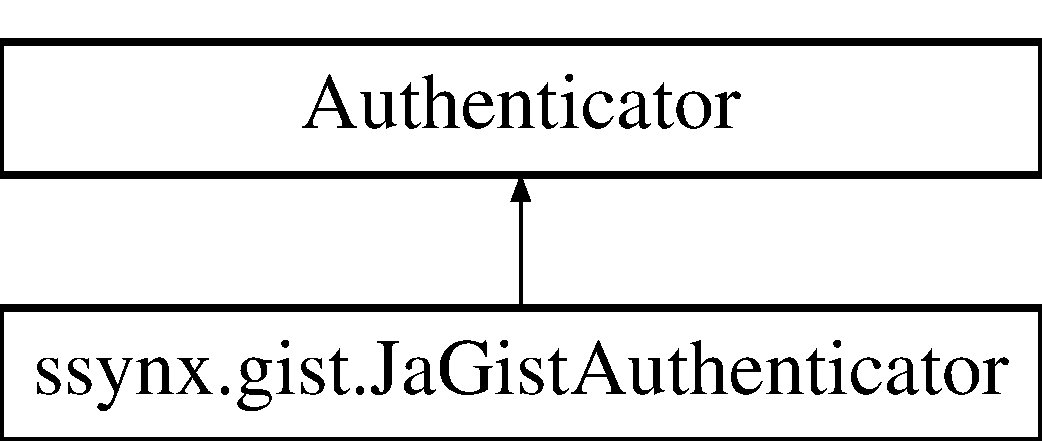
\includegraphics[height=2.000000cm]{classssynx_1_1gist_1_1JaGistAuthenticator}
\end{center}
\end{figure}
\subsection*{Public Member Functions}
\begin{DoxyCompactItemize}
\item 
\mbox{\Hypertarget{classssynx_1_1gist_1_1JaGistAuthenticator_aa0df6163fc01539bc1caacd31411ef99}\label{classssynx_1_1gist_1_1JaGistAuthenticator_aa0df6163fc01539bc1caacd31411ef99}} 
{\bfseries Ja\+Gist\+Authenticator} (final String username, final String password)
\end{DoxyCompactItemize}
\subsection*{Protected Member Functions}
\begin{DoxyCompactItemize}
\item 
\mbox{\Hypertarget{classssynx_1_1gist_1_1JaGistAuthenticator_a2f1dbfe031425fd44e635634b669f575}\label{classssynx_1_1gist_1_1JaGistAuthenticator_a2f1dbfe031425fd44e635634b669f575}} 
Password\+Authentication {\bfseries get\+Password\+Authentication} ()
\end{DoxyCompactItemize}


The documentation for this class was generated from the following file\+:\begin{DoxyCompactItemize}
\item 
src/main/java/ssynx/gist/Ja\+Gist\+Authenticator.\+java\end{DoxyCompactItemize}

\hypertarget{classssynx_1_1gist_1_1NewGist}{}\section{ssynx.\+gist.\+New\+Gist Class Reference}
\label{classssynx_1_1gist_1_1NewGist}\index{ssynx.\+gist.\+New\+Gist@{ssynx.\+gist.\+New\+Gist}}
\subsection*{Public Member Functions}
\begin{DoxyCompactItemize}
\item 
\mbox{\Hypertarget{classssynx_1_1gist_1_1NewGist_a2f0d270f3c86424e9928a2986e2d0660}\label{classssynx_1_1gist_1_1NewGist_a2f0d270f3c86424e9928a2986e2d0660}} 
{\bfseries New\+Gist} (final String description, final boolean is\+Public, final String filename, final String content)
\item 
\mbox{\Hypertarget{classssynx_1_1gist_1_1NewGist_a9336a2e1ec4a6d3c2ef6ad6f17cc6b43}\label{classssynx_1_1gist_1_1NewGist_a9336a2e1ec4a6d3c2ef6ad6f17cc6b43}} 
{\bfseries New\+Gist} (final String description, final boolean is\+Public, final File file)  throws I\+O\+Exception 
\item 
\mbox{\Hypertarget{classssynx_1_1gist_1_1NewGist_a3e7f317440b171171291f83661e268d4}\label{classssynx_1_1gist_1_1NewGist_a3e7f317440b171171291f83661e268d4}} 
void {\bfseries add\+File} (final String filename, final String content)
\item 
\mbox{\Hypertarget{classssynx_1_1gist_1_1NewGist_a729bad36788560e4a46f49515a997c30}\label{classssynx_1_1gist_1_1NewGist_a729bad36788560e4a46f49515a997c30}} 
void {\bfseries add\+File} (final File file)  throws I\+O\+Exception 
\item 
\mbox{\Hypertarget{classssynx_1_1gist_1_1NewGist_a5e9bd2f807725243f0c81d15c52b0948}\label{classssynx_1_1gist_1_1NewGist_a5e9bd2f807725243f0c81d15c52b0948}} 
String {\bfseries to\+String} ()
\end{DoxyCompactItemize}


The documentation for this class was generated from the following file\+:\begin{DoxyCompactItemize}
\item 
src/main/java/ssynx/gist/New\+Gist.\+java\end{DoxyCompactItemize}

\hypertarget{classssynx_1_1gist_1_1JaGist_1_1PerformGist}{}\section{ssynx.\+gist.\+Ja\+Gist.\+Perform\+Gist Class Reference}
\label{classssynx_1_1gist_1_1JaGist_1_1PerformGist}\index{ssynx.\+gist.\+Ja\+Gist.\+Perform\+Gist@{ssynx.\+gist.\+Ja\+Gist.\+Perform\+Gist}}
\subsection*{Static Public Member Functions}
\begin{DoxyCompactItemize}
\item 
\mbox{\Hypertarget{classssynx_1_1gist_1_1JaGist_1_1PerformGist_a31c3c40744cd0bd733f37d2f72391391}\label{classssynx_1_1gist_1_1JaGist_1_1PerformGist_a31c3c40744cd0bd733f37d2f72391391}} 
static \hyperlink{classssynx_1_1gist_1_1Gist}{Gist} {\bfseries create} (final \hyperlink{classssynx_1_1gist_1_1NewGist}{New\+Gist} gist)
\item 
\mbox{\Hypertarget{classssynx_1_1gist_1_1JaGist_1_1PerformGist_a641d3eb04fd6eea90852a09e161b20ef}\label{classssynx_1_1gist_1_1JaGist_1_1PerformGist_a641d3eb04fd6eea90852a09e161b20ef}} 
static \hyperlink{classssynx_1_1gist_1_1Gist}{Gist} {\bfseries edit} (final \hyperlink{classssynx_1_1gist_1_1EditGist}{Edit\+Gist} gist)
\item 
\mbox{\Hypertarget{classssynx_1_1gist_1_1JaGist_1_1PerformGist_aec33fe3614d0862f4280ee32feb2b558}\label{classssynx_1_1gist_1_1JaGist_1_1PerformGist_aec33fe3614d0862f4280ee32feb2b558}} 
static boolean {\bfseries star} (final String id)
\item 
\mbox{\Hypertarget{classssynx_1_1gist_1_1JaGist_1_1PerformGist_aa54ceda956caacdaee38a0a28ef533ea}\label{classssynx_1_1gist_1_1JaGist_1_1PerformGist_aa54ceda956caacdaee38a0a28ef533ea}} 
static boolean {\bfseries unstar} (final String id)
\item 
\mbox{\Hypertarget{classssynx_1_1gist_1_1JaGist_1_1PerformGist_afdc5bac2396bf40be8746bc9da384365}\label{classssynx_1_1gist_1_1JaGist_1_1PerformGist_afdc5bac2396bf40be8746bc9da384365}} 
static \hyperlink{classssynx_1_1gist_1_1Gist}{Gist} {\bfseries fork} (final String id)
\item 
\mbox{\Hypertarget{classssynx_1_1gist_1_1JaGist_1_1PerformGist_afaeacc6d2571c0f6f545f62def8b62f8}\label{classssynx_1_1gist_1_1JaGist_1_1PerformGist_afaeacc6d2571c0f6f545f62def8b62f8}} 
static boolean {\bfseries delete} (final String id)
\end{DoxyCompactItemize}


The documentation for this class was generated from the following file\+:\begin{DoxyCompactItemize}
\item 
src/main/java/ssynx/gist/Ja\+Gist.\+java\end{DoxyCompactItemize}

%--- End generated contents ---

% Index
\backmatter
\newpage
\phantomsection
\clearemptydoublepage
\addcontentsline{toc}{chapter}{Index}
\printindex

\end{document}
